\chapter{Evaluation}\label{chapter:evaluation}

\guidance{%
  This is where Assessors will be looking for \textbf{signs of success} and for
  \textbf{evidence of thorough and systematic testing}. \textbf{Sample output},
  tables of timings and photographs of workstation screens, oscilloscope traces
  or circuit boards may be included.\\
  As with code, voluminous examples of sample output are usually best left to
  appendices or omitted altogether.\\
  There are some obvious questions which this chapter will address. \textbf{How
  many of the original goals were achieved? Were they proved to have been
  achieved? Did the program, hardware, or theory really work?}\\
  Assessors are well aware that large programs will very likely include some
  residual bugs. It should always be possible to demonstrate that a
  \textbf{program works in simple cases} and it is instructive to
  \textbf{demonstrate how close it is to working in a really ambitious case}.\\
}

\prechapter{%
  Here, the project's resounding success, in relation its aims (as listed in
  Section~\ref{intro:aims}), will be justified. A comparison with existing
  tools will demonstrate the advantages of this project over existing tools
  (those mentioned in Subsection~\ref{prep:coqtools}). Sample output will be
  shown and the interesting insights they provide will be explained.
}%

\begin{figure}[tbp]

  \raggedright
  This project aims to:

  \begin{itemize}
  \item represent Coq libraries as Neo4j graph databases, which wil involve
    \begin{itemize}
    \item exploring and choosing the correct model
    \item converting and extending existing code to output CSVs
    \item writing new programs to extract extra information \\
        (omitted from other, existing tools)
    \item writing new programs to automate database creation; and to
    \end{itemize}

  \item create a library of Neo4j queries, intended
    \begin{itemize}
    \item to highlight the structure of and relationship between proof-objects
    \item by coalescing and implementing several graph-related metrics.
    \end{itemize}
  \end{itemize}

  \hrule%
  \bigskip
  \caption{Aims of the Project}\label{fig:aims}

\end{figure}

\section{Features}\label{eval:compare}

For convenience, the aims of the project, as listed in
Section~\ref{intro:aims}, are reproduced above, in Figure~\ref{fig:aims}.
Within the first major bullet-point (representing Coq libraries as Neo4j
databases), the latter three aims (of adapting, extending and writing new
programs to output CSV, extracting extra information and automating database
creation) were exposited in the~\nameref{chap:impl} chapter.

So, to assess the first aim of the project (exploring and choosing the
correct model), all of the programs listed in
Subsection~\ref{prep:coqtools},~\nameref{prep:coqtools}, are compared
side-by-side in Table~\ref{table:features}, in which this project comes out
favourably.

\subsection{Other Tools}

\begin{table}[p]
  \centering

  \begin{tabular*}{\textwidth}{@{\extracolsep{\fill}} rcccccccccc}

    \toprule

    & \rot{Source Code} & \rot{Hyperlinks} & \rot{Precise Kinds}
    & \rot{Constr. \& Types~~} % for vertical space after 'Types'
    & \rot{Type Sig.} & \rot{Module depend.} & \rot{Graphical rep.}
    & \rot{Interactivity} & \rot{Statistics} & \rot{Object depend.} \\

    \midrule

    Coqdoc    & \Y & \Y & \Y & \Y & \Y & \N & \N & \N & \N & \N \\
    Coqdep    & \N & \M & \N & \N & \N & \Y & \Y & \N & \N & \N \\
    CoqSerAPI & \N & \N & \N & \N & \N & \N & \N & \Y & \Y & \N \\
    dpdgraph  & \N & \N & \M & \N & \N & \N & \Y & \N & \N & \Y \\
    Project   & \M & \Y & \Y & \Y & \Y & \Y & \Y & \Y & \Y & \Y \\

    \bottomrule

  \end{tabular*}

  \medskip
  \Y\  Has feature \hfill \N\ Does not have feature \hfill \M\ Can be extended to support it

  \bigskip
  \caption{Comparison of Features}\label{table:features}

\end{table}

The features chosen for comparison reflect the strengths of each tool
considered.

Bundle with Coq, coqdoc produces \textbf{hyperlinked source code} meaning
details such as the \textbf{precise kinds} of a proof-object, the
\textbf{constructors of a type} and the \textbf{type signatures} are immediately
visible; hence those 5 dimensions were included.  Also include in a Coq system
is coqdep: a tool for modelling \textbf{module-level dependencies} that can
output a \texttt{dot} file to present it \textbf{graphically}.

Coq Serialised (S-expression) API is an \textbf{interactive} IDE communication
protocol with facilities for gathering some basic \textbf{statistics}. Here,
interactive is used to mean that information is not presented all at-once,
\emph{statically}, but can instead be queried dynamically at run-time. An
example of a static dispaly is Figure~\ref{fig:static}; it shows a medium-sized
Coq library as ouput by dpdgraph.

\begin{figure}[p]

  \centering
  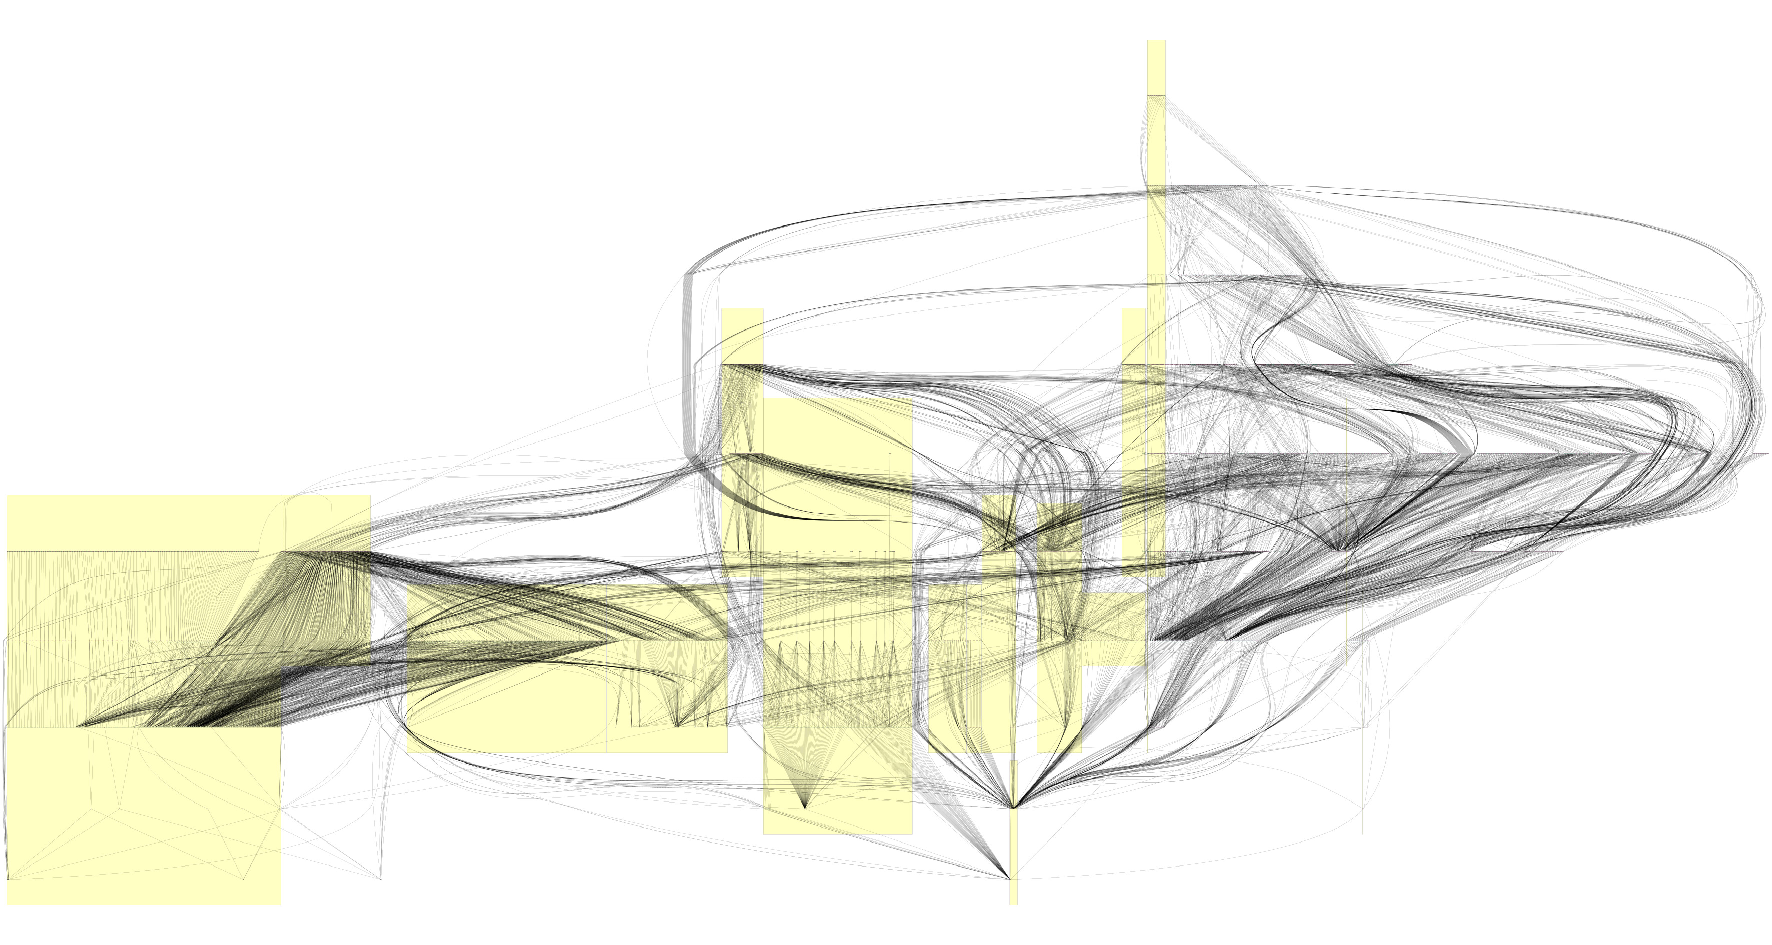
\includegraphics[width=\textwidth, page=1]{img/static-CAS-small.pdf}
  \caption{Static Output of dpdgraph (using \texttt{dpd2dot}) on
    \href{https://github.com/Timothy-G-Griffin/CAS}{CAS}}\label{fig:static}

\end{figure}

In principle, coqdep and dpdgraph can also support some degree of interactivity,
with support from other tools (which translate \texttt{dot} files to interactive
JavaScript), although this is rarely done.  What dpdgraph does do well is model
\textbf{object dependencies}, with some scope for distinguishing precise kinds
and displaying information graphically.

\subsection{This Project}

It is clear from the table that this project either supports, or can support,
every feature supported by other tools. However, it is important to note, that
in many cases, this project does not simply match the feature, but exceeds it in
ways described next.

Linking to source code could be supported by modifying either the model,
database or JavaScript visualisations (outuput by the library of queries) to
link to the relevant webpages output by coqdoc. So, a user could switch between
a graphical overview and a detailed inspection at will.

Whenever a node is visible, it can be expanded to see the nodes it depends on,
so in that sense, it supports hyperlinks, though, unlike hyperlinks, such
expansion is done in place, thus retaining the \emph{context} of its use.

Thanks to the \emph{kind} and \emph{subkind} labels, the project supports
precise kinds.  Also, any (co-)inductive type can, via the
\texttt{CONSTRUCTED\_BY} relation, be expanded to see its constructors.

Due to the \emph{type} property, each object's type is also visible. For a proof
object, its type is a statement of the actual theorem being proved, hence this
feature is incredibly important when coming to grips with a mathematical theory.
Crucially, it is a \emph{fully expanded} type signature, making explicit any
assumptions introduced (perhaps hunderds of lines prior in the source code) into
the environment.

Module dependencies are set with the query in Listing~\ref{lst:moddep} by use of
the \texttt{CONTAINS} relation.  Interactivity is achieved through the Neo4j
browser interface and the JavaScript visualisations; statistics are achieved
through the library of queries; graphical representations by both. An important
limitation of CoqSerAPI is that its statistics are (at the time of writing)
simply three counters, whereas this project offers many sophisticated graph
metrics and the ability (through a queriable database) to gain \emph{any} sort
of information a user is interested in.

\begin{listing}[p]%

\caption{Query to set Module Dependencies}\label{lst:moddep}

  \begin{minted}{cypher}
    MATCH (a)-[:USES]->(b),
          (src:module)-[:CONTAINS]->(a),
          (dst:module)-[:CONTAINS]->(b)
    WHERE src.objectId <> dst.objectId
    CREATE UNIQUE (src)-[r:DEPENDS_ON]->(dst)
    SET r.weight = coalesce(r.weight, 0) + 1
    RETURN r
  \end{minted}

\end{listing}

And finally, object dependencies are at the heart of this project: by using a
Neo4j graph database, we can understand and manipulate this relation in a much
more flexible and scalable manner than any visualisation can manage.

\section{Performance}

This project could have all the features any user could ever want but if it ran
so slowly that nobody would have the patience to use it, then it would be wrong
to consider it as having met its aims. So, here, this project's execution time
is compared to most of the tools from the previous section. Although it is
slightly slower than other existing tools, this can be directly accounted for
by its larger feature set and increased flexibility.

\subsection{Setup}

To evaluate timings, the Coq (8.6) Standard Library was used, due to its sheer
size (564 modules, 5823 definitions, 23,892 proofs). For coqdoc and coqdep,
Coq's Makefiles were modified to measure execution time using bash's \emph{time}
command. At the time of writing, CoqSerAPI's statistics were not fully/usably
implemented, so it was not measured. For dpdgraph, seprate measurements were
taken for outputting a \texttt{dpd} file and converting that file to a dot
Format. A similar approach~\textendash of measuring database creation (model
output, CSV translation and data import) and library analysis
separately~\textendash was taken for this project, so that the comparison was as
fair as possible. Each set of timings was repeated five times (with the
exception of \texttt{dpd2dot} which, at nearly \emph{27 minutes}, was not
repeated because of time and system-usability constraints).

\begin{figure}[tp]
\centering
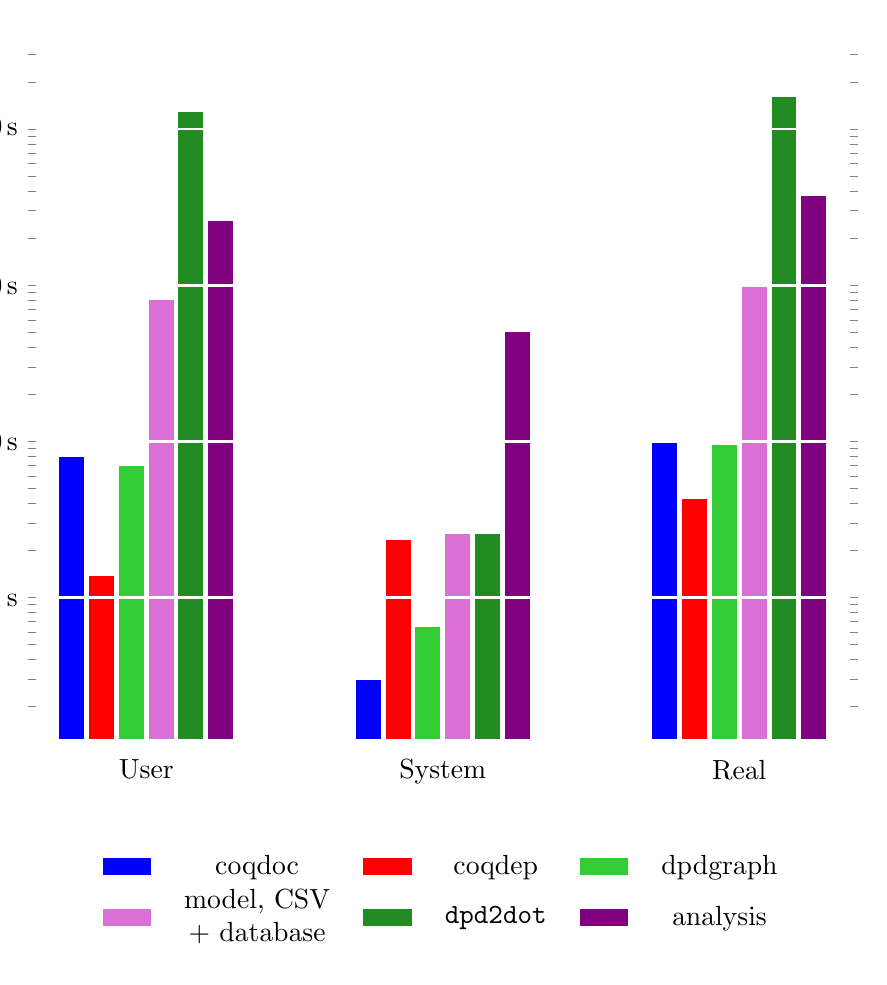
\begin{tikzpicture}[trim axis left]
	\begin{axis}[
    % width of chart
    width=\textwidth,
    % no box, below chart, horizontal
		legend style={%
      draw=none,
      at={(0.5,-0.15)},
      anchor=north,
      legend columns=3,
      column sep = 1em,
      cells={align=center},
    },
    % value above position on bar chart
		ybar=0.5ex, % bar chart, with inter-bar spacing of 1ex
    log ticks with fixed point,
    yticklabel={\pgfmathparse{pow(10,\tick-3)}\pgfmathprintnumber[fixed]{\pgfmathresult}}\,s, % N ms along y-axis
    symbolic x coords={User,System,Real},
		xtick=data,
    axis line style={opacity=0}, % hide y axis
    major tick style={draw=none}, % no ticks
    ymode=log, % log scale for y
    log basis y = {10}, % log base 10
		enlarge x limits=0.20, % spacing on x axis
    bar width=2ex,
    ymajorgrids, % rows of lines
    major grid style={white, line width=1pt},
    axis on top,
	]

  % Coqdoc
  \addplot [area legend, style={Blue,fill=Blue,mark=none}]
    coordinates {(User,7877) (System,0295) (Real,10007)};

  % Coqdep
  \addplot [area legend, style={red,fill=red,mark=none}]
    coordinates {(User,1361) (System,2299) (Real,4257)};

  % dpdgraph
  \addplot [area legend, style={LimeGreen,fill=LimeGreen,mark=none}]
    coordinates {(User,6872) (System,0645) (Real,9392)};

  % creation
  \addplot [area legend, style={Orchid,fill=Orchid,mark=none}]
    coordinates {(User,79254) (System,2521) (Real,98157)};

  % dpd2dot
  \addplot [area legend, style={ForestGreen,fill=ForestGreen,mark=none}]
    coordinates {(User,1272249) (System,2516) (Real,1588303)};

  % analysis
  \addplot [area legend, style={violet,fill=violet,mark=none}]
    coordinates {(User,255912) (System,49569) (Real,371881)};

  \legend{coqdoc,coqdep,dpdgraph,{model, CSV\\+ database},\texttt{dpd2dot},analysis}

	\end{axis}

\end{tikzpicture}

\caption{Comparison of Execution Times}\label{fig:exectimes}
\end{figure}

\subsection{Results}

Figure~\ref{fig:exectimes} shows the results of the comparison, as broken-down
by bash's time command into time spent in user-code, system calls and overall.
Note that the data is presented on a \emph{logarithmic} scale. Immediately
we see coqdoc takes very little time to run, approximately 10 seconds and coqdep
even less at around 4 seconds, which, considering their purely lexical
approaches, is to be expected.

So it is somewhat surprising that dpdgraph runs just as quickly as coqdoc. The
increase in system time can be explained by the 14MB \texttt{dpd} file output by
dpdgraph. Although at first it appears that there is an order-of-magnitude
slowdown with this project, more detailed examination explains precisely
\emph{what} occurs during database creation and where ineffeciencies lie.

\subsection{Inefficiencies}

Setting up a graph database from scratch can take some time. Assuming a Coq
project is already compiled, the following steps need to take place:

\begin{enumerate}
  \item\label{step:gen} generating file with a list of all the modules to be
    examined (15 ms),
  \item\label{step:compile} compile that file using the Coq compiler (12.6 s),
  \item\label{step:dpd2csv} convert the output \texttt{dpd} file to CSV files (72.7 s),
  \item create a Neo4j database from those CSV files (12.8 s)
\end{enumerate}

When steps~\ref{step:gen} and~\ref{step:compile} are taken on their own, we see
that the changes to accomodate a more detailed model resulted in a 25\%
slowdown, which is acceptable given this is a stress-test and the difference is
on the order of seconds. Creating a database from CSV files takes a similar
amount of time, also acceptable given the size of the graph (31,088 nodes and
850,434 edges).

So, the real bottleneck is step~\ref{step:dpd2csv}: converting \texttt{dpd}
files to CSV. During execution, \texttt{dpd2} reads in a 25MB \texttt{dpd} file
and outputs two CSV files of size 7MB (nodes) and 8MB (edges), so IO is likely
to be a factor, as is reconstructing the graph in memory. Outputting to
\texttt{dpd} was done to facilitate easy extension with other tools. It is
likely that outputting a CSV directly would have resulted in being able to
bypass this phase altogether, though, from a software-engineering
point-of-view, the trade-off there is increased coupling.

\subsection{Graph Analysis \& Visualisation}

Once a graph is created (whether it be in the form of \texttt{dpd} file or a
dabtabase) the last step is to \emph{use} the data by analysing and visualising
it. Here, this project shows a significant improvement over \texttt{dpd2dot}.

At nearly \emph{27 minutes}, its execution time dwarfs the analyses carried out
by this project. Whereas \texttt{dpd2dot} converted the output 13MB \texttt{dpd}
file to a 24MB dot file, in about one-quarter of the time, an R script was able
to run (a) PageRank and closeness centrality algorithms over all proofs and
defintions and (b) output \emph{8} different 9MB visualisations of the data.
Analyses took less than a minute; visualisations ranged from 20 to 90 seconds.

It should be noted that \texttt{dpd2dot} did not do graph \emph{layout}: it just
split the graph into subgraphs (based on modules) and assigned a colour and label
to each node (based on their properties). Converting the dot file to a viewable
format (e.g.\ a scalable vector-graphic or SVG) is up to another tool (that
being said, the command \texttt{dot -Tsvg} to produce an SVG visualisation had to
be cancelled after failing terminate within a few \emph{hours}).

\section{Library of Queries}\label{sec:libeval}

Within the second major bullet-point (creating a library of Neo4j queries), the
second aim (of coalescing and implementing graph-related metrics) was dealt
with in the~\nameref{chap:impl} chapter. To assess the first aim (of
highlighting the structure of and relationship between proof-objects), the
library will be shown to work on the small case of a Coq Regular-Expression
package and on the large case of the project's moonshot, the Odd Order Theorem.

\begin{figure}[p]
\centering
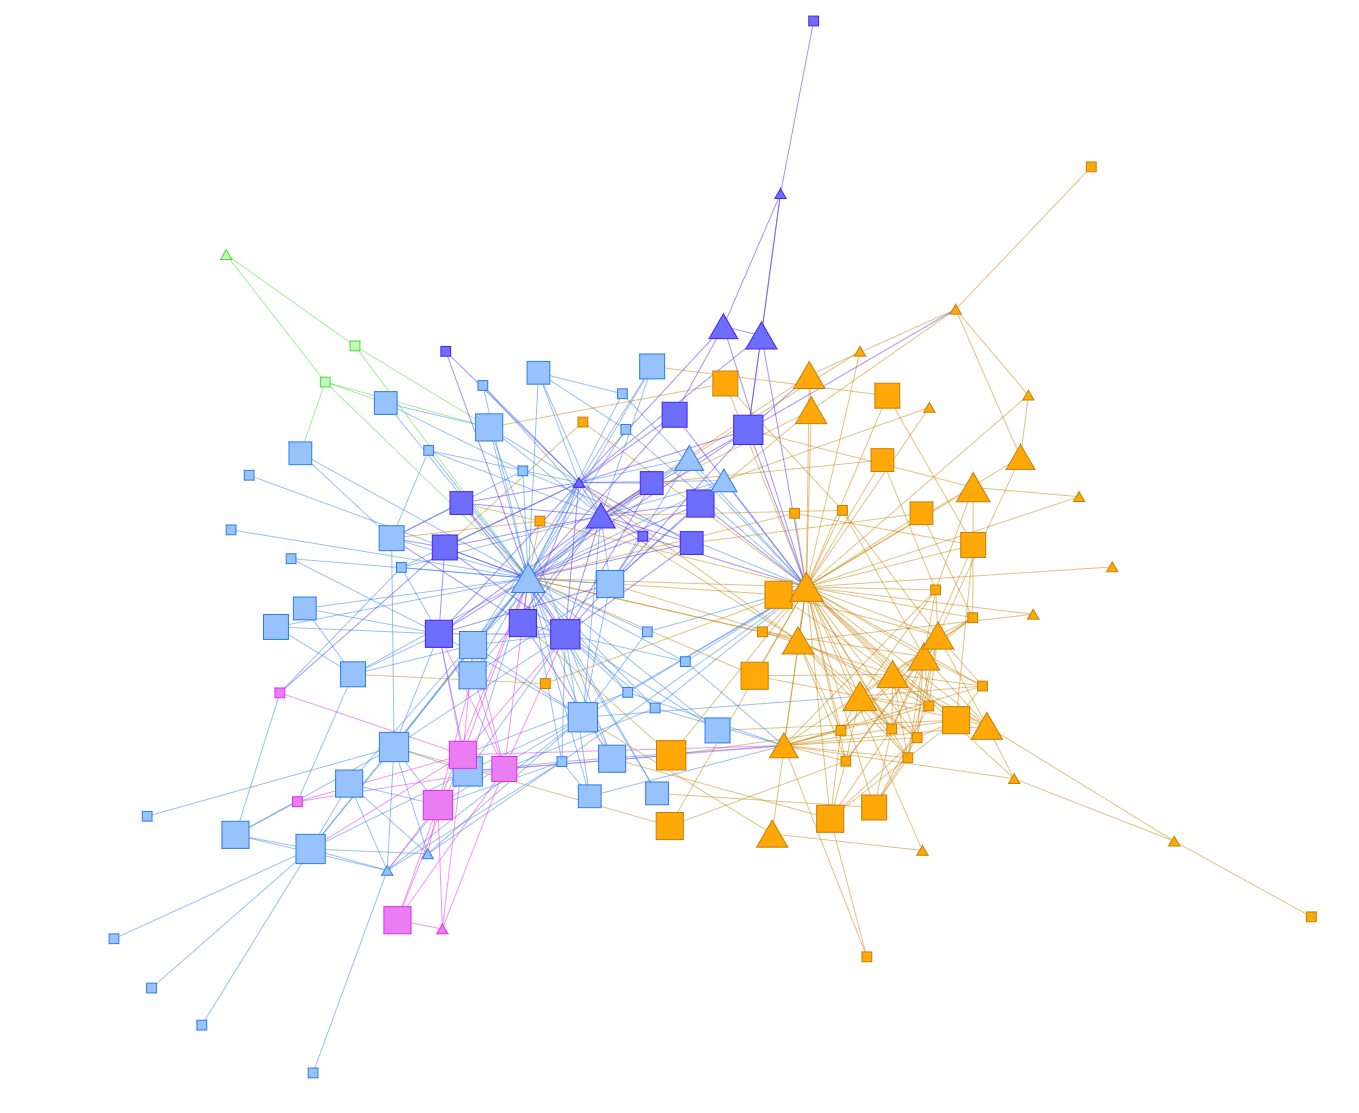
\includegraphics[width=0.8\textwidth]{img/regexp/direct.png}
\caption{Force-directed with Betweenness Centrality}\label{fig:regexp:direct}
\end{figure}

\begin{figure}[p]
\centering
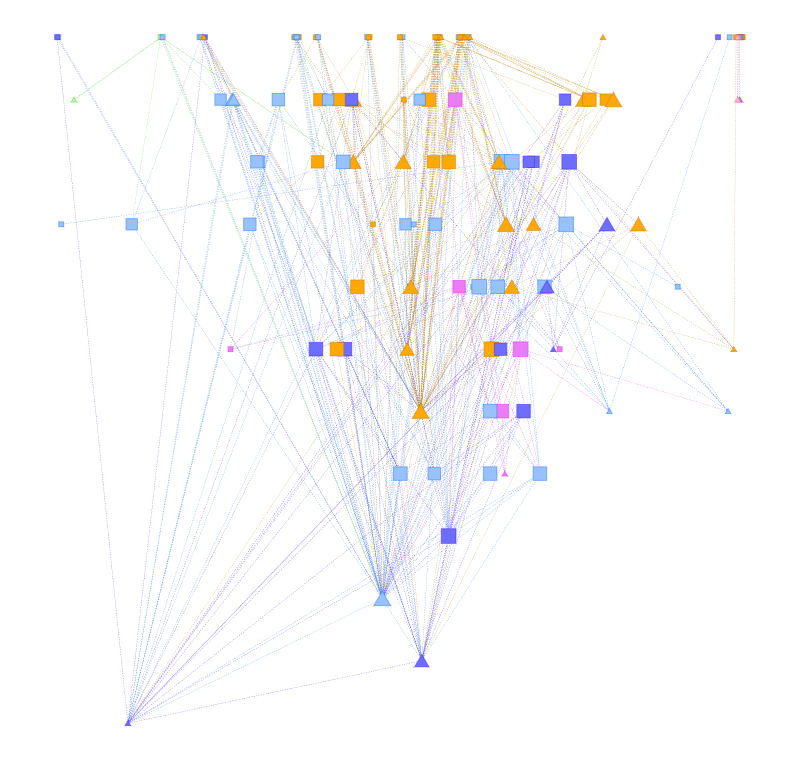
\includegraphics[width=0.8\textwidth]{img/regexp/hierarchical.png}
\caption{Hierarchical with Betweenness Centrality}\label{fig:regexp:hier}
\end{figure}

\begin{figure}[tp]
  \begin{minipage}{0.5\textwidth-0.5em}
    \centering
    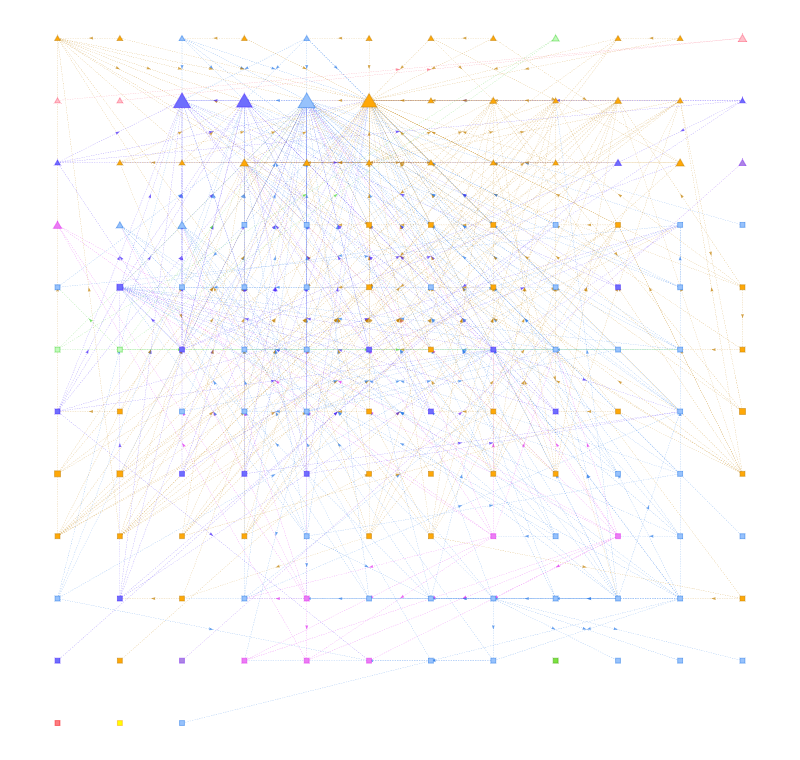
\includegraphics[width=\textwidth]{img/regexp/grid.png}
    \caption{Grid Layout with PageRank}\label{fig:regexp:grid}
  \end{minipage}%
  \hspace{1em}%
  \begin{minipage}{0.5\textwidth-0.5em}
    \centering
    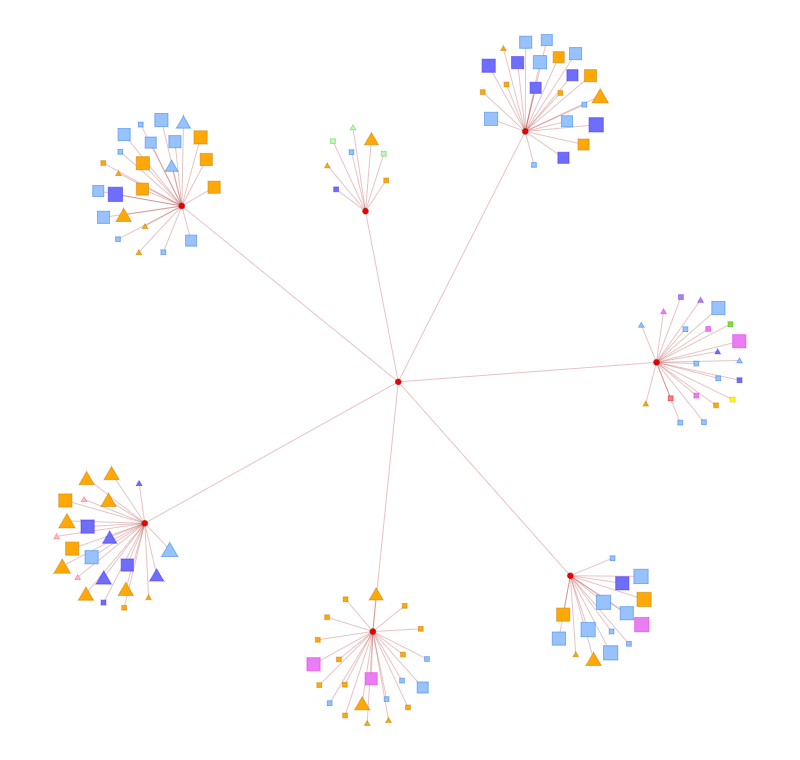
\includegraphics[width=\textwidth]{img/regexp/module.png}
    \caption{Force-directed with Modules}\label{fig:regexp:module}
  \end{minipage}
\end{figure}

\subsection{Small: CoqRegExp}

For this package, PageRank, betweenness centrality, modularity clustering,
hierarchical layout, grid layout and force-directed layout produced the most
aesthetically pleasing and insightful results. All graphs show only definitions
(shown as triangles, reminiscent of the $\triangleq$ symbol sometimes used for
definitions) and proofs (shown as squares, reminiscent of the end-of-proof
$\square$ symbol), except for Figure~\ref{fig:regexp:module} which also includes
modules (as circles).

\subsubsection{Direct}

Figure~\ref{fig:regexp:direct} shows a force-directed visualisation. The size of
the nodes corresponds to betweenness centrality scores (split up into 10
logarithmically equal-width buckets). Colours correspond to groups assigned by modularity
clustering. Edges represent the \texttt{USES} relation; edge-directions
(source-uses-destination) are omitted for clarity since they generally point
toward the the center of a cluster.

We see that modularity clustering largely corresponds to the how a human might
group nodes visually: two major clusters with a few, smaller clusters.
Intuitively, the \glblue{light blue} cluster represents \glblue{\emph{executable
functions}}; the \gorange{orange} cluster represents \gorange{\emph{proofs of
correctness}}; the \glpurple{light purple} cluster represents proofs using the
definition of \glpurple{string length}; the \glgreen{light green} cluster
represents proofs involving \glgreen{converting strings to regular-expressions};
the \gviolet{violet} cluster represents proofs relating to \gviolet{nullable
strings}. The node at the center of the light blue cluster is a function which
computes whether a given regular-expression matches a given string; the node at
the center of the yellow cluster defines what it means for two
regular-expressions to be equal.

\subsubsection{Hierarchical}

As far as insights are concerned, we see that this enables us to get a
high-level view of the threads of thought in the theory. We can see how these
threads develop by looking at Figure~\ref{fig:regexp:hier}.  Here, a Sugiyama
layout is used (the direction of edges always points downwards). If nodes were
partially ordered according the \texttt{USES} relation (destination $<$ source
if and only if source \texttt{USES} destination) then this layout ensures that
if a node (destination) is \emph{below} another node connected to it (source)
then the source \texttt{USES} destination.

Applied to mathematical theories, this layout is essentially a visual
study-guide, a plan for how to best tackle the material. It can be applied to
subgraphs, refined by declaring the maximum depth or the lowest layer to include
and filtered based on the kind or importance of a node.

\subsubsection{Grid and Modules}

Given a strategy for how to approach the material, knowing how important each
section is can be useful for gauging how much time to spend on understanding it.
As indicators of importance, measures of centrality are a useful way to do
precisely that. Figure~\ref{fig:regexp:grid} represents PageRank through node
size on uniform grid, useful for visually determining relative importance.

And finally, Figure~\ref{fig:regexp:module} shows the proofs and defintions
with modules, where edges represent the \texttt{CONTAINS} relation. We see that
the modules at the right and near the center (named Utility, Includes and Char
respectively) have very few important nodes (as determined by betweenness
centrality). Each module has two main parts: those relating to
\glblue{executable functions} those relating to \gorange{proofs of correctness},
occasionally accompanied by a few definitions/proofs on \gviolet{nullability}
or \glpurple{string length}.

\subsubsection{Insights}

Without studying even \emph{one line} of source code, we have been able to gleam
an intuitive and impressively detailed conceptual-scaffolding of this theory of
regular-expressions. A user can use the library of queries to futher explore the
theory or jump into reading the source code with a much better idea of how
the different pieces of the puzzle come together.

\subsection{Large: Odd Order Theorem}

For the Odd Order Theorem, betweenness centrality (for node size), modularity
clustering (for node colour), hierarchical layout, grid layout, circular layout
and force-directed layout produced the most aesthetically pleasing and
insightful results. As before, only definitions (shown as
triangles/$\triangleq$) and proofs (shown as squares/$\square$ symbol) are
shown, except for Figure~\ref{fig:oot:module} which also includes modules (as
circles). New to this section, edges are coloured. Unless a figure is stated as
being flipped, the colour of an edge is the same colour as its source (user);
otherwise, it is the same colour as its destination (used).

This Coq package closely follows the structure of the source material:
Peterfalvi~\cite{peterfalvi2000oot} and Bender \&
Glauberman~\cite{bender1994oot}. Each section (chapter) in the original books is
a file/module in the Coq package; each definition/lemma/proof/corollary
corresponds to the same in the books. Following the convention in the Coq
package, Bender \& Glauberman will henceforth be abbreviated to BG and
Peterfalvi to PF.

\subsubsection{Overview}

Starting with a force-directed visualisation of nodes,
Figure~\ref{fig:oot:direct} highlights five major groups: \gdblue{dark blue},
\gpink{pink}, \gyellow{yellow}, \gpurple{purple}, \gdgreen{dark green} and
\gmagenta{magenta}; it shows that modularity clustering largely agrees with the
layout. Clear connections are visible between each of the groups, with a central
group showing a mix of almost all groups.

Figure~\ref{fig:oot:module} shows the same nodes in their module structure; of
note is the remarkable consistency of clusterings (based \emph{only} on the
\texttt{USES} edges between proofs and definitions) to fall within their
grouping the moudule boundaries defined by the \texttt{CONTAINS} relation.

Figures~\ref{fig:oot:circleflip} and~\ref{fig:oot:grid} show a circular (with
edge directions flipped) and grid layout of the Coq package. An advantage of the
flipped circular layout is that is can show which groups are being used the most
and how; an advantage of the grid layout is one can get an intuition what
proportion of definitions/proofs belong to a certain group.

\subsubsection{Groups}

%  5 - Pink:        BG 1-6,AB
%  4 - Dark blue:   PF 1,2,5,6,7
%  3 - Purple:      BG 7,10,12,14,16 -- PF 3,4,8
%  1 - Dark green:  BG 7,8,9,10,11,12,13,15 -- PF 8,9,10,11,12,13,14,15
%  2 - Magenta:     BG 15,16 -- PF (1,8,9) 10,11,12,13,14
%  7 - Light green: BG (4,7) 10
% 20 - Yellow:      PF 3 - CyclicT Iso Reflection
%  6 - Light blue:  Stripped Odd Order

We can begin to uncover some of the meaning by looking at the \modulegraph.  The
seven \gpink{pink} circles (six near the center, one at the far left) are BG
sections 1-6 and Appendices A/B. As the first sections, one would assume they
lay the groundwork for the rest of the theory; this assessment is backed-up by
the \hiergraph. Of about 36 rows in the \gridgraph, 6 of them are \gpink{pink}.
All sections except BG 5 \emph{surround} the central cluster in the
\directgraph.  The slight red diagonal on the right of the \circlegraph\ shows
sparser connections than most of the other groups.

Similarly, the modules containing mostly \gdblue{dark blue} nodes are the early
chapters (1,2,5,6,7) of PF, expositing mostly foundational material (as seen in
the \hierflipgraph) but in an extremely directed and linear fashion (as seen in
the \hiergraph).  They are a dense group (as shown by the left of the
\circlegraph) and occupy about 6 rows in the \gridgraph. Apart from PF 2 (right)
and 5 (left), they are tightly-woven into the center of the \directgraph.

\gpurple{Purple} and \gdgreen{dark green} share the later sections (7-16) of BG.
Where they differ is PF: \gpurple{purple} covers PF 3,4 \& 8 whereas
\gdgreen{dark green} covers PF 8-15. This difference is apparent in
\hyperref[fig:oot:hier]{both} \hyperref[fig:oot:hierflip]{hierarchical} graphs:
\gpurple{purple} nodes occupy the middle of the graphs but green nodes form
a steep line from top to bottom. Both are clustered in the center of the
\directgraph, with the exception of PF 4 as two \gpurple{purple} clusters to the
bottom-left. They dominate the \circlegraph\ and the \gridgraph, occupying
around 8 rows each.

\gmagenta{Magenta} forms the later sections of both BG (15-16) and PF (8-14), so
it comes as little surprise that it occupies the upper half of both
\hyperref[fig:oot:hier]{both} \hyperref[fig:oot:hierflip]{hierarchical} graphs.
Even though it only constitutes about two rows in the \gridgraph, we see its
striking bands on the \circlegraph\ because of how often its results are used by
other nodes in the final sections (15-16) of PF.

Other miscellaneous groups include \glblue{light blue} (a self-contained,
stripped down proof of just the Odd Order Theorem from first principles),
\gyellow{yellow} (an entire excursion to proving PF Theorem 3.5) and
\glgreen{light green} (primarily BG 10).

\subsubsection{Insights}

With some context about the composition of the theory, we can now examine
\hyperref[fig:oot:hier]{both} \hyperref[fig:oot:hierflip]{hierarchical} graphs
in a bit more detail to see truly understand what they reveal about this
monumental Coq package and the books it encodes.

Figure~\ref{fig:oot:hier} shows the hierarchical, Sugiyama layout.  A
consequence of this algorithm is that nodes are placed \emph{closest to their
first use}, usually done as a heuristic to minimise edge crossings. Intuitively,
one can think of this approach as the lazy/ultra-efficient student who only
studies a particular definition/proof \emph{just before} it is needed by some
other part of the text (or like call-by-need evaluation in a non-strict
programming language).

As such, swapping the direction of the edges \emph{does not} simply flip the
layout vertically, as Figure~\ref{fig:oot:hierflip} shows. One could conjecture
that Figure~\ref{fig:oot:hier} shows how mathematics is \emph{developed} (a
narrow foundation, top-down refinement, creating proofs/definitions as and when
needed, several independent lines of thought) and Figure~\ref{fig:oot:hierflip}
shows how mathematics is presented (a broad base of \emph{all} the groundwork
that will be needed first, followed by a bottom-up, rapidly developing, linear
argument which uses the base extensively).

% Direct & Modules
\begin{figure}[p]
\centering
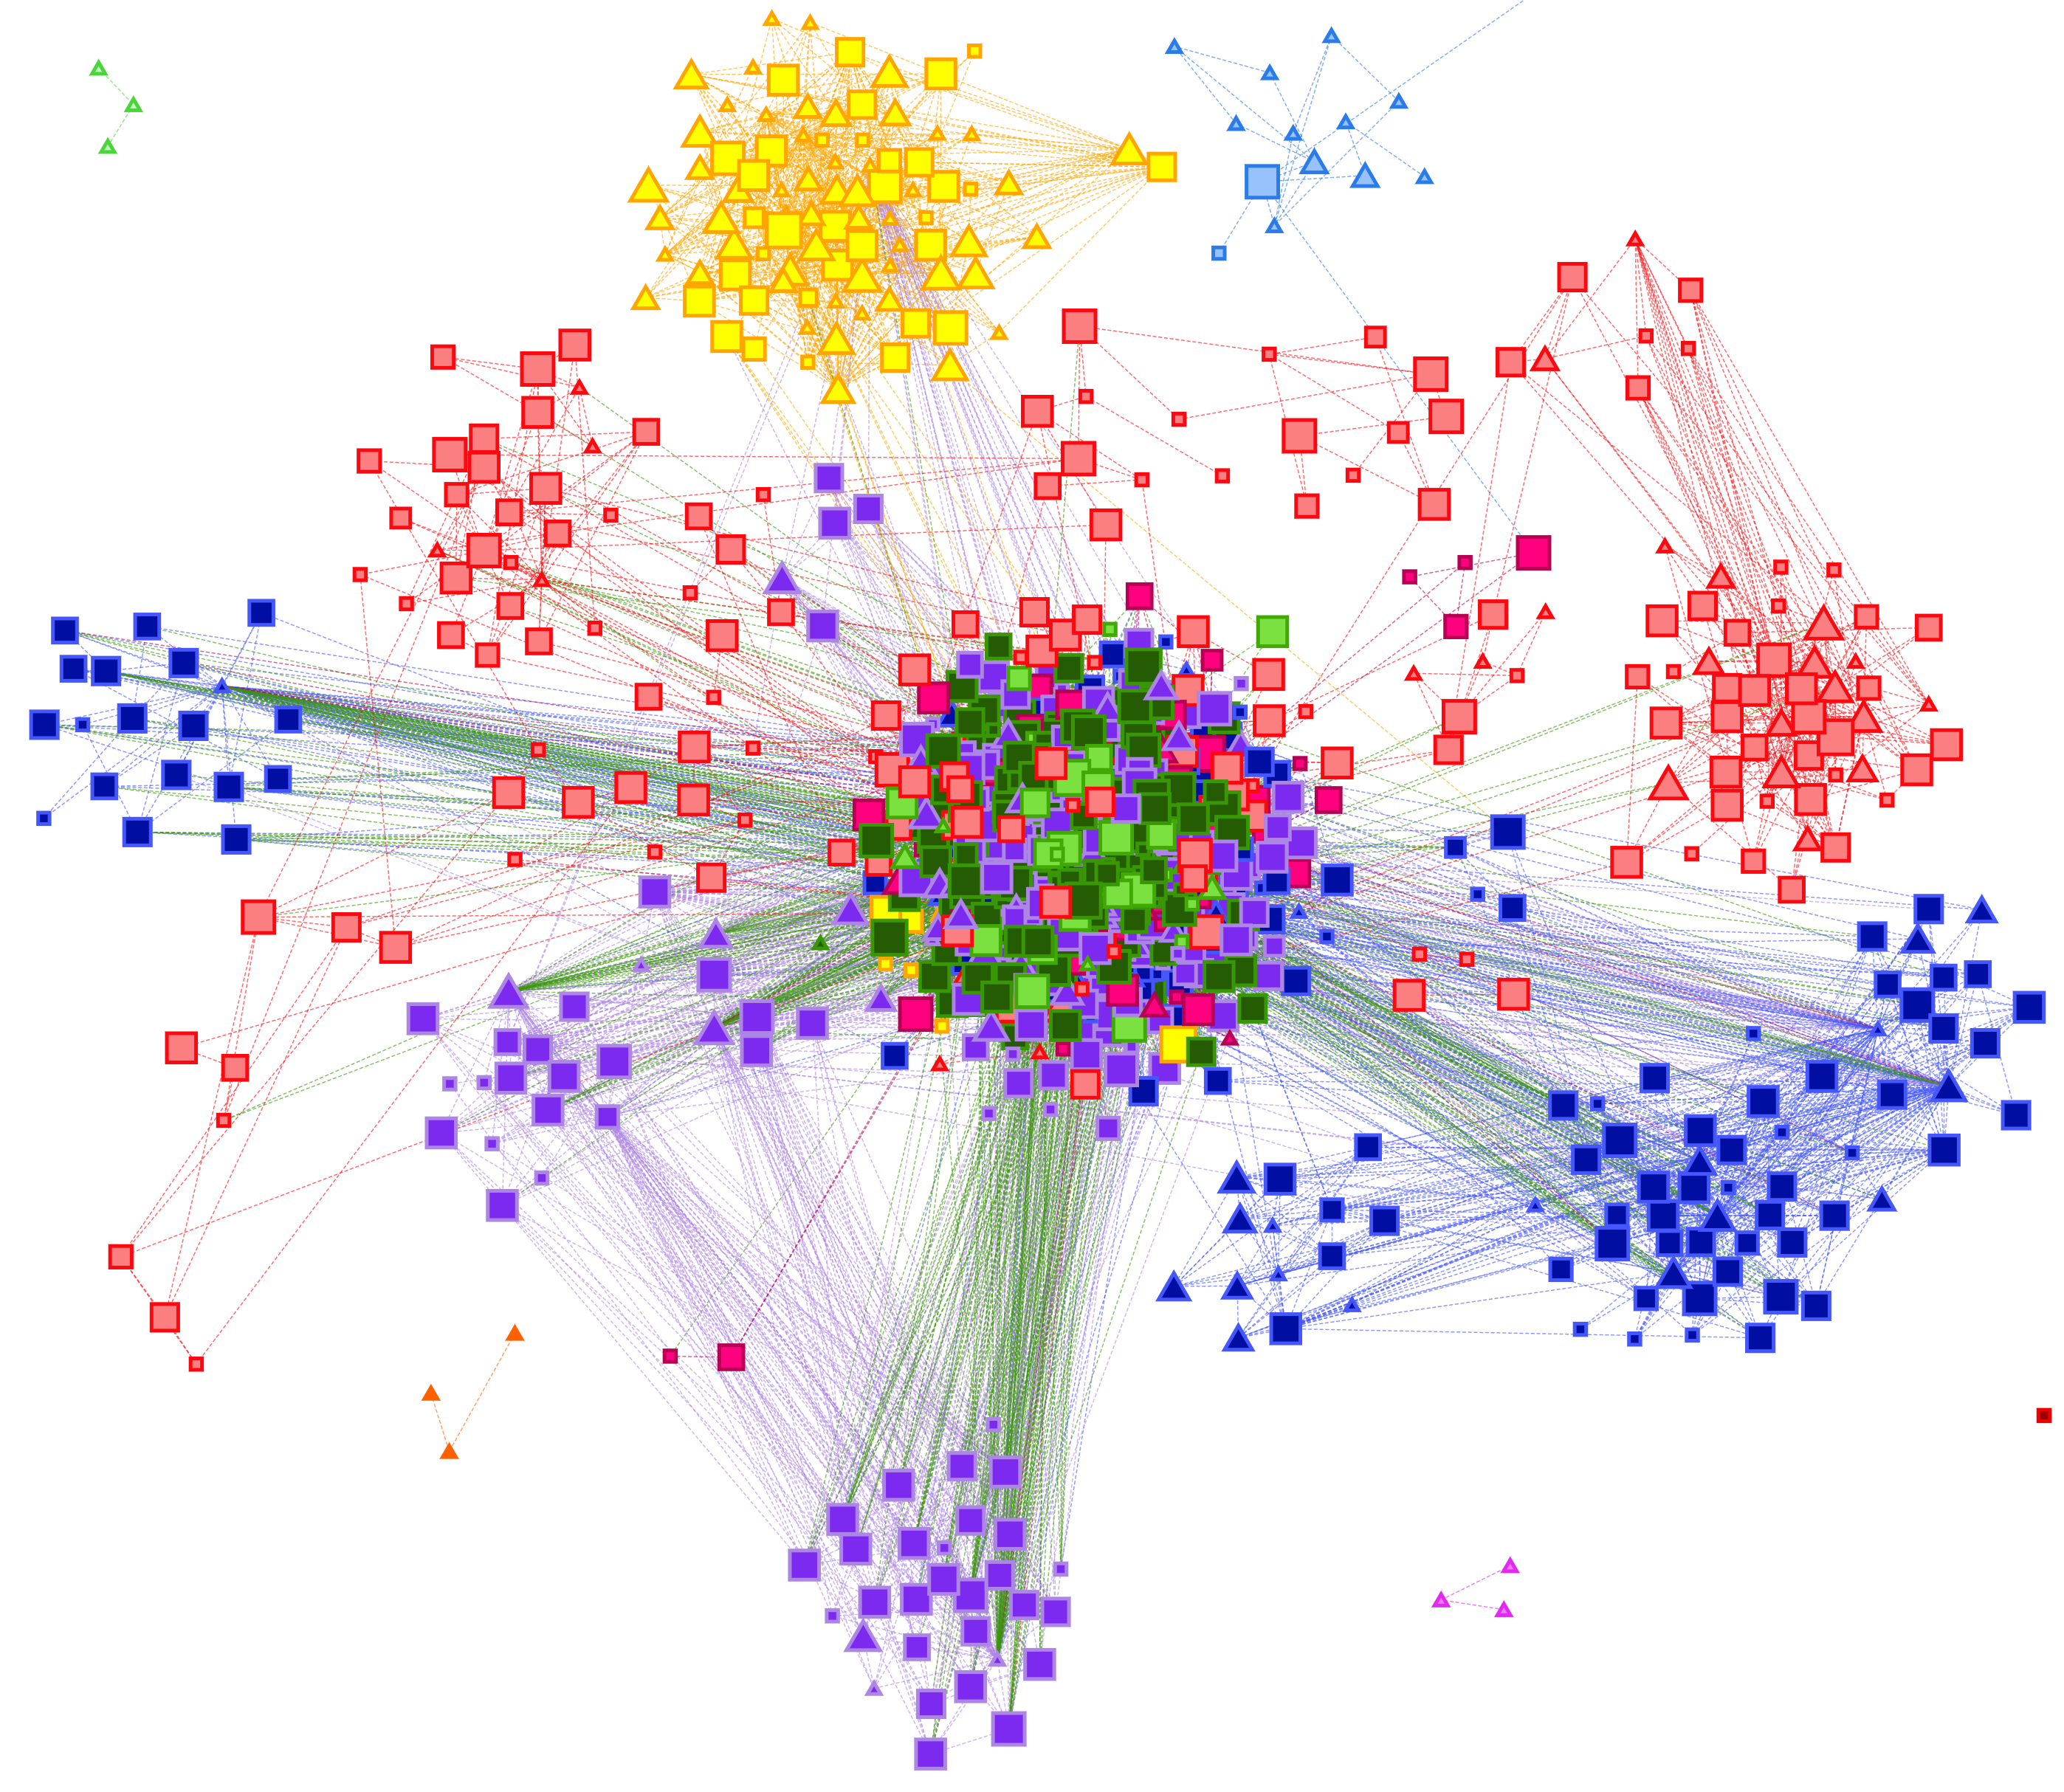
\includegraphics[height=0.45\textheight]{img/oot/direct}
\caption{Force-directed (some nodes omitted for clarity)}\label{fig:oot:direct}
\end{figure}

\begin{figure}[p]
\centering
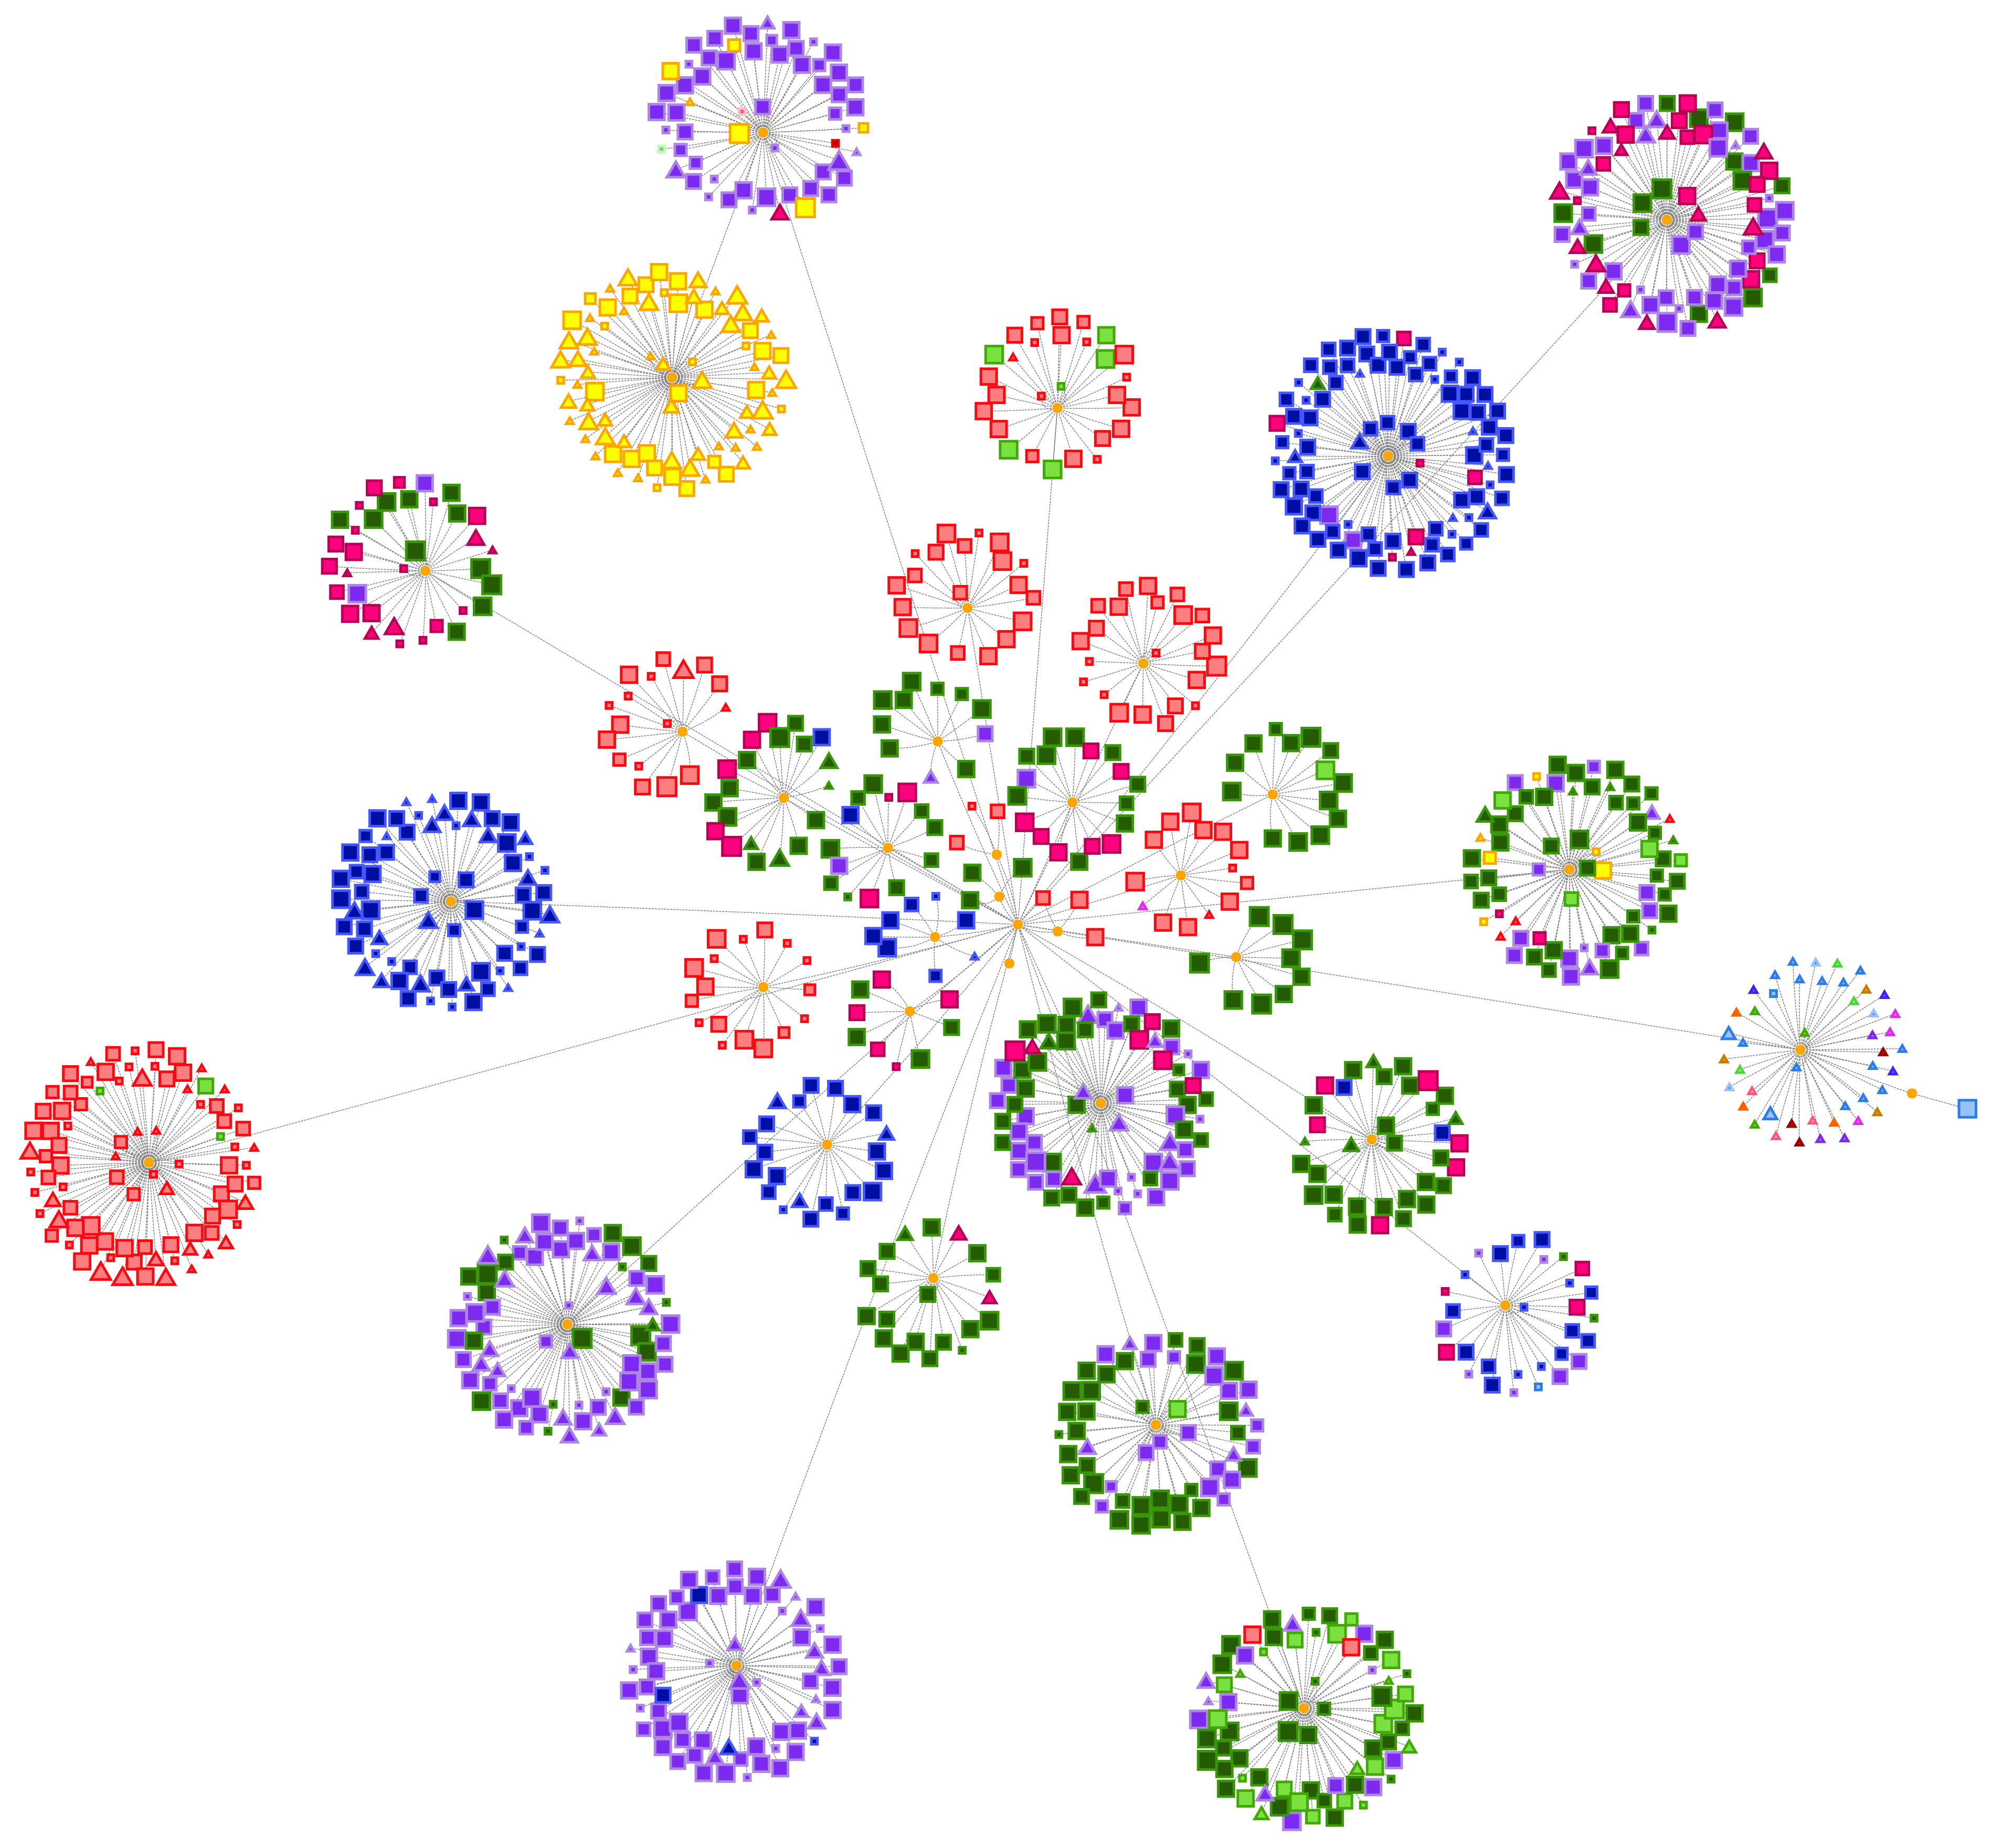
\includegraphics[height=0.45\textheight]{img/oot/modules}
\caption{Modules}\label{fig:oot:module}
\end{figure}

% Hierarchicals
\begin{figure}[p]
\centering
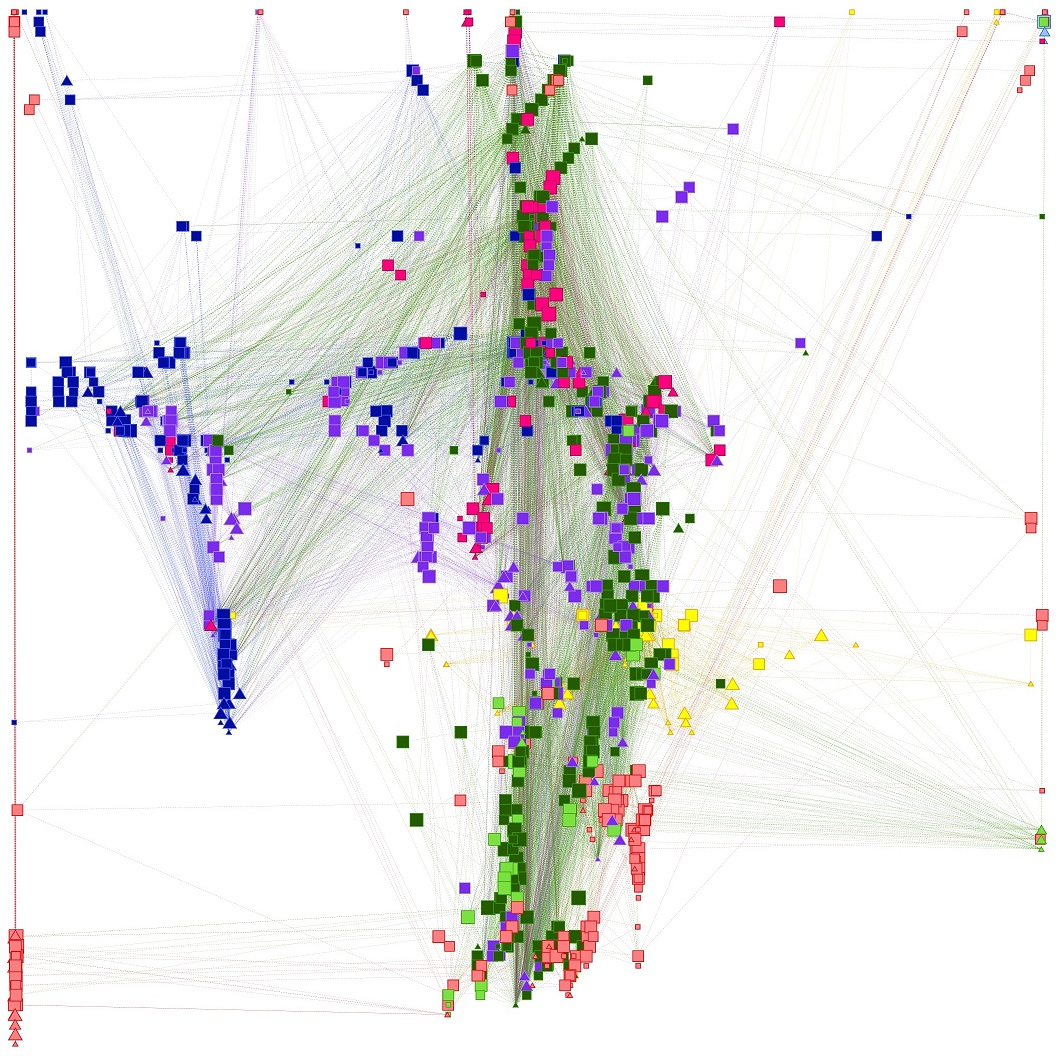
\includegraphics[height=0.45\textheight]{img/oot/hierarchical}
\caption{Hierarchical}\label{fig:oot:hier}
\end{figure}

\begin{figure}[p]
\centering
\reflectbox{\rotatebox[origin=c]{180}{%
  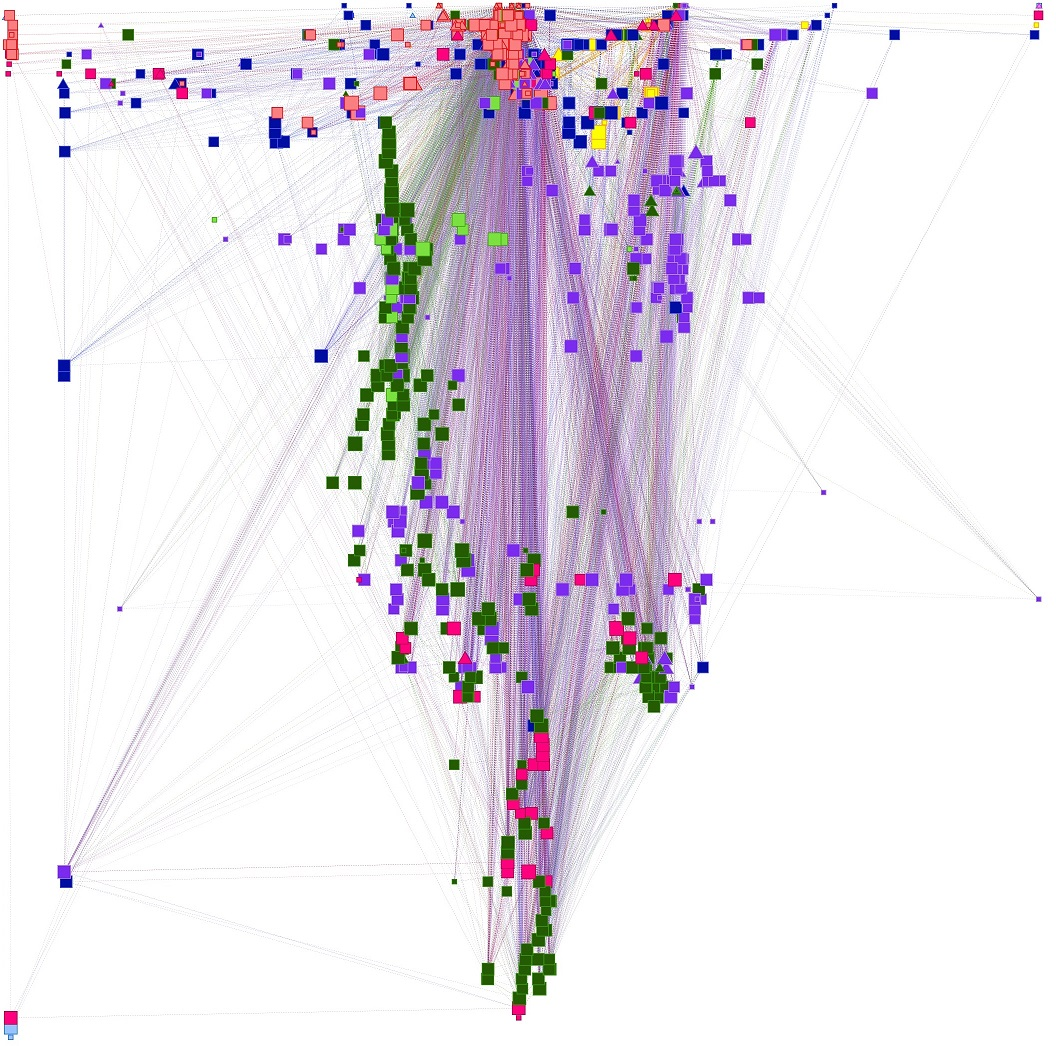
\includegraphics[height=0.45\textheight]{img/oot/hierarchical_flipped}}}
\caption{Hierarchical Flipped}\label{fig:oot:hierflip}
\end{figure}

% Circular & Grid
\begin{figure}[p]
\centering
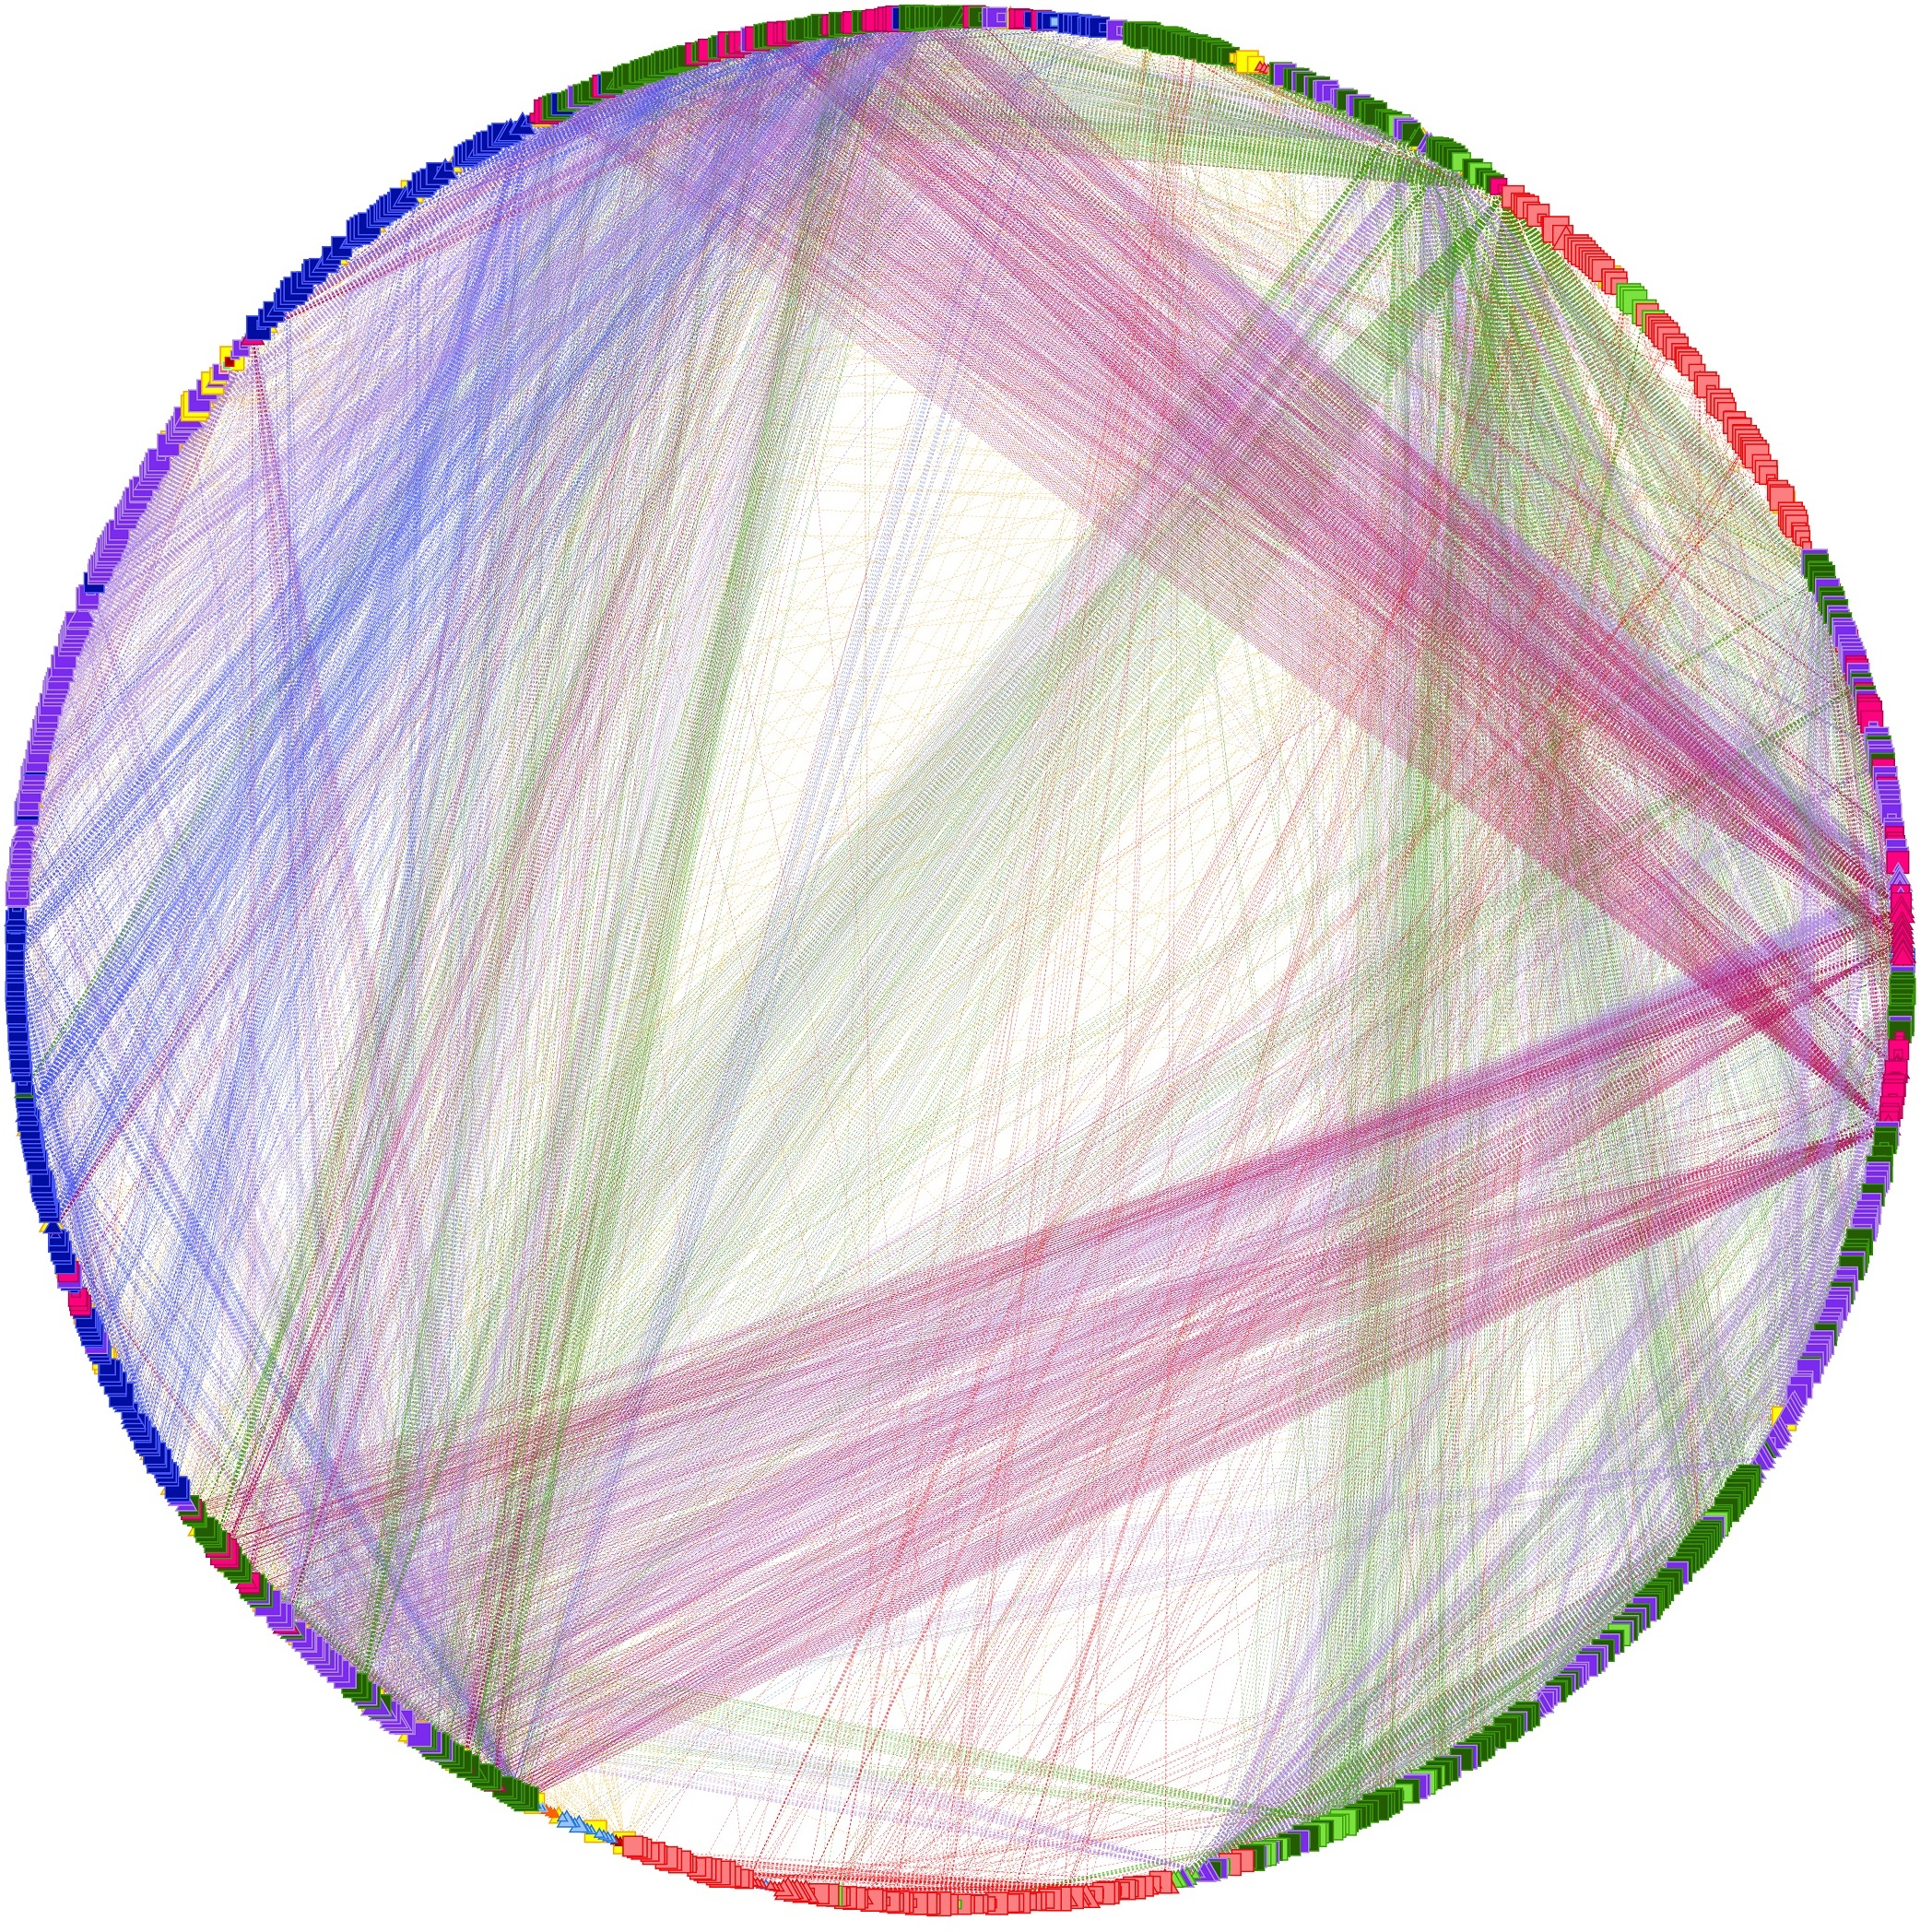
\includegraphics[height=0.45\textheight]{img/oot/circular_flipped}
\caption{Circular Flipped}\label{fig:oot:circleflip}
\end{figure}

\begin{figure}[p]
\centering
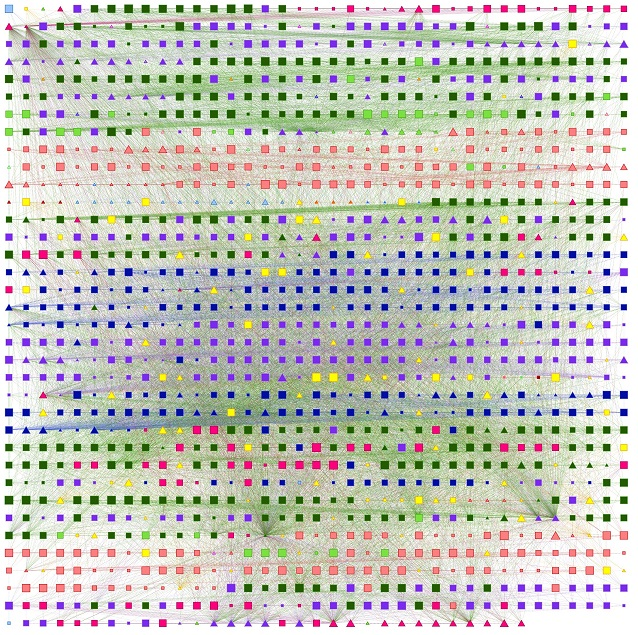
\includegraphics[height=0.45\textheight]{img/oot/grid}
\caption{Grid}\label{fig:oot:grid}
\end{figure}

\newpage%
\section{Summary}

To assess the two major aim of this project (choosing the correct model and
being able to gain insights into mathematical theories), its features,
performance and output were examined in detail. For its features, a systematic
comparison with other, existing tools of a similar purpose, showed this project
went above and beyond what existing tools offer. For its performance, a similar
comparison of execution times showed this project to be slightly slower, but
still acceptable and usable for even the most extreme of cases. For its output,
two Coq packages, each representing a mathematical theory, were explained via
the insights gained from using this project on them.
